\documentclass[a4paper,14pt]{memoir}
\usepackage[danish]{babel}
\usepackage[utf8]{inputenc}
\usepackage{hyperref}
\usepackage{ebgaramond}
\usepackage{graphicx}
\usepackage{amsmath}
\newtheorem{paastand}{Påstand
}
\title{Matematik og andre fiktioner}
\author{Hans Hüttel \and Simon Kongshøj}
\date{Foråret 2020}

\begin{document}

\maketitle

\chapter{Om denne bog}

Denne lille bog handler om eksistens og matematik -- ikke om menneskets eksistens, men om matematiske objekters eksistens eller mangel på samme.

\section{Hvem vi skriver til og hvorfor}

Vores målgruppe er som udgangspunkt alle, der spekulerer på hvad matematik skal gøre godt for. Nogle skal i gang med at lære matematik på en videregående uddannelse. Nogle har haft underlige eller dårlige oplevelser med matematik tidligere, og har måske overbevist sig om at de ikke har ``matematikhjerne''. Nogle er bare nysgerrige.

En af de erfaringer, vi har gjort os, er at en kombination af nogle mærkelige kulturelle forestillinger om matematik og den måde nogle matematikere taler på gør at mange studerende tror at matematik er noget nærmest mystisk og overnaturligt, som ikke rigtig har noget med virkeligheden at gøre. Med til denne tanke hører ofte en forestilling om at forståelse for matematik kræver en helt særlig---muligvis medfødt---gave, som kun et fåtal er i besiddelse af.

\section{Hvad er matematik \emph{egentlig}?}

Vores budskab er, at det forholder sig helt anderledes, end mange regner med. Virkeligheden kom først. Matematikken er en fiktion, vi bruger for at tale om virkeligheden; en fiktion der tillader at ignorere virkelighedens væld af detaljer for bedre at få et mentalt greb om den. Men det er ikke en fiktion der er grebet ud af den blå luft; den fortæller en historie om regelmæssigheder i virkeligheden. Det er mennesker der har udviklet den og bliver ved med at udvikle den---og selvom mange af matematikhistoriens store skikkelser unægteligt var exceptionelt begavede, så kræver matematisk forståelse ikke nogen exceptionel gave. Det kræver bare at man er menneske.

Men hvad er egentlig matematikkens grundlag, hvis matematik er en fiktion? Det har været udgangspunkt for utallige slagsmål blandt matematikere og filosoffer og har dannet grundlag for flere store "ismer" i matematikkens filosofi. Vores morale er, at hele dette slagsmål mellem "ismerne" er -- fiktivt.

De seneste års udvikling inden for datalogi, et fag vi begge færdes i, tyder på at de forskellige "ismer" ikke er konkurrerende religioner, men komplementerende syn på matematikkens grundlag. De kan og skal eksistere samtidig. Det store bevis (om vi så må sige) for at det er sådan, er de computerbaserede bevisassistenter, som nu er ved at vinde frem. Det er datalogien, der er med til at give matematikken dens grundlag nu.

\section{Hvad står der i denne bog?}

I denne bog vil vi give nogle enkle eksempler på de vigtige fiktioner, som findes i matematikken.

Undervejs vil vi vende tilbage til tallene, fordi tallene er en af de vigtigste og mest grundlæggende fiktioner i matematik. Her er vi inspireret af Rantzaus bog \emph{Alle tiders tal} \cite{rantzau}, der er en usædvanligt rig og spændende bog om tallenes historie.
\chapter{Fiktioner}

Når nu vil påstår, at matematik er en fiktion, er det vigtigt for os først at grundlægge begrebet.

\section{Et ord fra latin}

Ordet \emph{fiktion} kommer selvfølgelig fra latin.

Den Danske Ordbog \cite{ordnet} angiver at ordet kommer

\begin{quote}
   fra latin \textsl{fictio} (genitiv -onis), afledt af latin \textsl{fingere} 'forme, opdigte' 
\end{quote}
 
og giver derefter en af betydningerne som
 
 \begin{quote}
     \ldots antagelse som fremsættes fordi den er hensigtsmæssig som filosofisk eller videnskabelig metode, uagtet den kan være falsk eller modsigelsesfuld
 \end{quote}
 
 Det er netop dén betydning, vi tager udgangspunkt i: At matematikkens begreber er antagelser, skabt af mennesker, fordi de er hensigtsmæssige. Og de vil ofte rumme usandheder, mangler og modsigelser. Arbejdet med at håndtere disse problemer, der er en vigtig del af matematikkens historie.
 
\section{Darth Vaders lyssværd}

Men lad os starte et helt andet sted end i matematikkens verden. Ordet \emph{fiktion} har nemlig også en anden betydning af ordet, nemlig \cite{ordnet}

\begin{quote}
    litteratur (fx roman og novelle), film el.lign. der beskriver helt eller delvis opdigtede personer og begivenheder
\end{quote}

Er påstanden 

\begin{quote}
    Darth Vader kæmper med et rødt lyssværd
\end{quote}
sand?

Det er den strengt taget ikke, for Darth Vader findes ikke, og lyssværd gør heller ikke. Men i den sammenhæng, vi alle sammen accepterer, når vi taler om Star Wars,  er påstanden faktisk sand. Skulle læseren være i tvivl, prøv da at se eller gense nogle af de gamle film. 

Der er et krav, som de to slags fiktioner har fælles, nemlig et krav om at være \emph{modsigelsesfri}. Hvis Darth Vader i nogle scener pludselig kæmpede med et grønt lyssværd, ville vi umiddelbart sige, at det var "forkert", også selv om vi godt ved, at Darth Vader er en fiktion konstrueret af George Lucas.

\section{Pallas Athene}

Eksisterer den græske gudinde Athene? Her vil de allerfleste nulevende mennesker sige nej.

\section{Eksisterer Google?}

Lad os gå lidt længere væk. Eksisterer Google?

For nogle vil svaret være, at ja, virksomheden Google eksisterer. Det gør den så egentlig ikke, thi den hedder faktisk Alphabet. 

Men hvad med søgemaskinen Google?

Hvis Google findes, så tvinges vi til at acceptere at Athene også  fandtes engang. Hun har ihvertfald haft mange ansatte og rådet over store samfundsinstitutioner.

Google og Athene findes, men er fiktioner. Fiktion er ikke er "usand" - mennesker bruger den til at forstå virkeligheden med, og dermed bruger de den også til at forme virkeligheden med. På samme måde med matematik.
Uanset om Athene findes eller ej, så har forestillingen om Athene faktisk formet verden. På samme måde som mange af de fiktive entiteter vi i dag har former verden i dag (og ikke kun i positiv retning).

\section{Tallene}

Tallet 3 findes heller ikke, i den forstand at vi ikke kan gå ud noget sted og kigge på det; der er ingen måleinstrumenter der kan vise os det, og det er ikke en del af tid og rum. Men i matematikkens fiktion findes det, og det har mange egenskaber vi kan tale om.

Men vi kan definere begrebet "tre". Den tyske matematiker og logiker Gottlob Frege talte om "tre" som den egenskab, alle samlinger af størrelsen tre har til fælles.

I næste kapitel vender vi tilbage til tallene.



\chapter{De naturlige tal}

Alle kender de naturlige tal, selv om man måske ikke ved, at de hedder netop dét. De naturlige tal er tallene
%
\[ 1, 2, 3, 4, 5, 6, 7, 8, 9, 10, 11 \ldots \]
%
Hvorfor kaldes de naturlige tal \emph{naturlige}? Begrebet er i al fald gammelt. Ordet dukker op i 1763 i \emph{The method of increments} af den engelske matematiker William Emerson, der taler om 
\begin{quote}
    To find the product of all natural numbers from 1 to 100 \ldots
\end{quote}
men der er også tidligere anvendelser, hvor matematikerne siger, at der er noget særligt "naturligt" ved netop denne slags tal.

Hvad er det, der er så naturligt her? Måske fordi der er tale om den fiktion om tal, der naturligt falder mennesker ind. Børn lærer at tælle, længe før de lærer om de negative tal, for slet ikke at tale om brøkerne.

Den store tyske matematiker Leopold Kronecker er kendt for at have sagt (i en korrespondance med sin kollega og landsmand Ferdinand Lindemann) at

\begin{quote}
    Die ganzen Zahlen hat der liebe Gott gemacht, alles andere ist Menschenwerk. 
\end{quote}

eller oversat til på dansk

\begin{quote}
    De hele tal har den kære Gud skabt, alt andet er menneskeværk.
\end{quote}

Kronecker mente således, at matematikken er menneskers værk -- en fiktion. Men hvem skabte de naturlige tal? Det var såmænd den italienske matematiker Giuseppe Peano.

\section{Peanos aksiomer}

\begin{figure}[h]
    \centering
    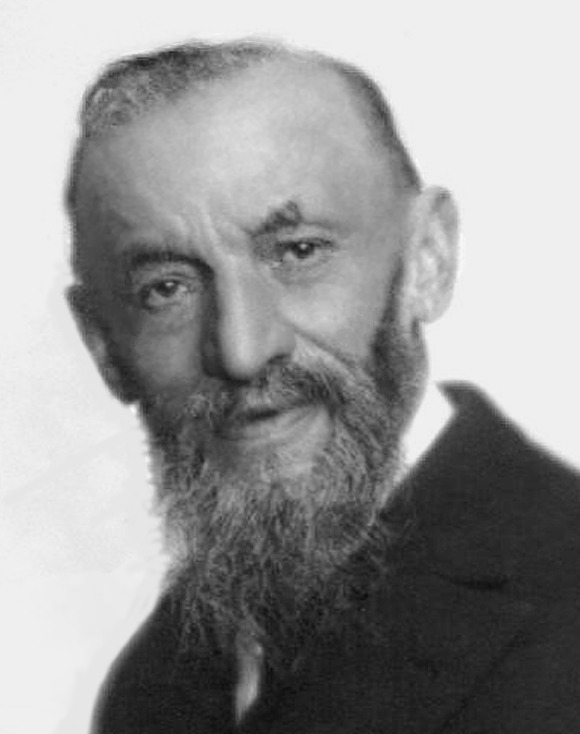
\includegraphics[width=6cm]{GiuseppePeano.jpg}
    \caption{Giuseppe Peano}
    \label{fig:peano}
\end{figure}

Den italienske matematiker Giuseppe Peano (1858-1932) gav en definition af de naturlige tal, der har vundet indpas i matematik, nemlig det, vi i dag kender som Peanos aksiomer. Peanos aksiomer fortæller os, at de naturlige tal er de tal, vi kan nå ved at starte ved $0$ og tælle opad. Og de lyder sådan:

\begin{enumerate}
    \item $0$ er et naturligt tal
    \item Hvis $n$ er et naturligt tal, er efterfølgeren $S(n)$ også et naturligt tal
    \item Der findes ikke andre naturlige tal end disse.
\end{enumerate}

Efterfølgerfunktionen $S$ skal man blot tænke på som et "flag" vi sætter foran. Ofte vil man skrive $n+1$ i stedet for $S(n)$, og det vil vi også af og til gøre i det følgende.

Tallet $2$ kan vi repræsentere som $S(S(0))$, dvs. ved at sætte $2$ $S$'er foran $0$. Og tallet $16$ kan vi på tilsvarende vis repræsentere som
%
\[ S(S(S(S(S(S(S(S(S(S(S(S(S(S(S(S(0))))))))))))))))\]
%
Læseren vil med lidt tålmodighed nemt kunne finde repræsentationen af $484719$.

\section{Addition}

Vi kender godt regningsarterne. Hvis vi vil definere addition, kan vi gøre det således.

\begin{enumerate}
    \item \label{plus-1} $0 + n = n$
    \item \label{plus-2} $S(n) + m = S(n+m)$
\end{enumerate}

Dette er endnu en fiktion om de naturlige tal.

\subsection{At vise at $2+2 = 4$}

Hvad er $2+2$? Husk at $2$ er $S(S(0))$. Så spørger vi, hvad $S(S(0)) + S(S(0))$ er. Her kan vi bruge vores fiktion om addition, undskyld vores definition af $+$.

Hvis vi sætter ind i betingelse \ref{plus-2}, får vi os at 
%
\[ S(S(0)) + S(S(0)) = S(S(0) + S(S(0)))  \]
%
og ved igen at sætte ind i betingelse \ref{plus-2}, får vi os at 
%
\[  S(S(0) + S(S(0))) = S(S(S(0 + S(0)))) \]
%
Så kan vi bruge betingelse \ref{plus-1}, og den giver os ved indsætning at
%
\[ S(S(S(0 + S(0)))) = S(S(S(S(0)))) \]
%
Så resultatet er $S(S(S(S(0))))$, dvs. tallet $4$. Med andre ord: Vi har nu vist at $2+2 = 4$.

\section{For alle naturlige tal gælder at \ldots}

Peano angav også en metode til at bevise, at en påstand gælder for alle naturlige tal. 

\begin{quote}
Lad $P$ være en påstand.
    \begin{enumerate}
    \item Hvis påstanden $P$ gælder for $0$
    \item Og hvis vi kan vise, at hvis påstand $P$ gælder for et naturligt tal $n$, da gælder $P$ også for $S(n)$    
\end{enumerate}
Da ved vi at påstanden $P$ gælder for alle naturlige tal
\end{quote}

Denne bevisteknik kalder man i dag for \emph{matematisk induktion}. Teknikken er meget ældre end Peano; den skyldes en anden italiener, Francesco Maurolico, der i sin bog \emph{Arithmeticorum libri duo} fra 1575 bruger matematisk induktion til at vise at summen af de første $n$ ulige tal:
%
\[ 1 + 3 + \cdots + (2n-1)  \]
%
er $n^2$. 

Matematisk induktion består i at vise at vores påstand gælder for det mindste naturlige tal, nemlig $0$ - det kalder vi for \emph{basistilfældet}. Og vi skal derefter vise, at påstanden bliver ved med at gælde, når vi giver os til at tælle -- det kalder vi for \emph{induktionsskridtet}.

Man kan også starte længere fremme i den naturlige talrække end ved $0$. Hvis man vil vise at en påstand $P$ gælder for alle naturlige tal der er større end eller lig $k$, skal vi bare vise at 

 \begin{enumerate}
    \item Påstanden $P$ gælder for $k$ (så $k$ er nu basistilfældet)
    \item Hvis påstanden $P$ gælder for et naturligt tal $n$, da gælder $P$ også for $S(n)$    
\end{enumerate}

Lad os se, hvad Maurolico gjorde, og lad os beskrive det, som Peano ville have gjort det.

Påstanden $P$ er altså at 
%
\[ 1 + 3 + \cdots + (2n+1) = n^2  \;\text{for}\; n \geq 1\]
%
Først skal vi vise basistilfældet, nemlig at summen af de første $1$ naturlige tal er $1^2$. Men det er oplagt, for $1 = 1^2$.

Så kommer skridtet. Vi skal vise, at hvis påstanden $P$ gælder for $n$, så gælder den også for $n+1$.

Påstanden $P$ gælder for $n$ præcis når
%
\[ 1 + 3 + \cdots + (2n-1) = n^2 \]
%
Det næste ulige naturlige tal efter er $(2n-1) + 2$. Så vi skal vise at
%
\[  1 + 3 + \cdots + (2n-1) + ((2n-1)+2) = (n+2)^2 \] 
%
Men betragt summen 
%
\[  1 + 3 + \cdots + (2n-1) + ((2n-1)+2)\] 
%
Den kan skrives som 
%
\[  (1 + 3 + \cdots + (2n-1)) + ((2n-1)+2) \] 
%
Hvis vi antager at påstanden $P$ gælder for $n$, har vi at
%
\[ 1 + 3 + \cdots + (2n-1) = n^2 \]
%
men så ved vi at
%
\[  (1 + 3 + \cdots + (2n-1)) +  ((2n-1)+2) = n^2 + ((2n-1)+2) \] 
%
Men 
\[ (n+1)^2 = n^2 + 2n + 1 \]
og
\[  n^2 + ((2n-1)+2) = n^2 +2n + 1 = (n+1)^2 \] 
hvilket afslutter beviset.

\section{Vores fiktion om addition ligner addition!}

En af de helt grundlæggende love, som skal gælde om addition, er at det er ligegyldigt i hvilken rækkefølge vi lægger tal sammen. Vi vil rigtig gerne have, at f.eks. $2+3 = 3+2$. Denne lov kalder man ofte for \emph{den kommutative lov}. 

Lad os prøve at vise at den kommutative lov gælder for de naturlige tal, dvs. at $m+n = n +m$ for alle naturlige tal $m$ og $n$.

Vi viser

\begin{paastand}
For ethvert naturligt tal $m$ gælder det, at det for ethvert naturligt tal $n$ gælder at $m + n = n + m$.
\end{paastand}

Dette er en påstand om alle naturlige tal $m$, så for at vise den, bruger vi matematisk induktion for $m$.

Først skal vi vise påstanden for $m = 0$, dvs. at $0+n=n+0$.

Men det er jo også en påstand om alle naturlige tal. Den hedder

\begin{paastand}\label{paa:to}
For alle naturlige tal $n$ gælder at $0+n=n+0$.
\end{paastand}

så den skal vises også. Så her skal vi også bruge matematisk induktion for at vise Påstand \ref{paa:to}.

Så lad os vise Påstand \ref{paa:to} først. Først skal vi vise, at $0+0=0+0$, men det gælder jo umiddelbart.

Så antager vi, at $0+n = n+0$ og skal med den antagelse i baglommen vise, at så gælder det også at $0 + (n+1) = (n+1) + 0$. Men $(n+1) + 0 = (n+0)+1$ ifølge vores definition af addition. Og da $n+0 = n$, må vi have at $(n+1) + 0 = n +1 $. Pr. definition af addition har vi at $0 + (n+1) = n+1$, og nu kan vi se, at påstanden gælder.

\section{\ldots men hvad med subtraktion?}

Når man har sagt plus, siger man også på et eller andet tidspunkt minus -- eller subtraktion, som det også kaldes.

Vi ved, at de naturlige tal ikke er \emph{lukket under} subtraktion. For $1-2$ er ikke et naturligt tal. Løsningen på det er enkel: Vi indfører de negative tal.

Så de negative tal er endnu en fiktion.
\chapter{Total fiktion i computeren}

\section{Tal og to-tal}

Når computere skal arbejde med tal, er de nødt til at repræsentere dem på en eller anden måde.

En repræsentation af et tal kalder man for en \emph{numeral}. Numeraler er dermed en fiktion om tal.

Normalt skriver vi i vore dage tal med numeraler fra det, vi kalder for titalssystemet. Tallet sytten skriver vi som $17$, for $17$ er summen af $1$ ti'er og $7$ enere. Tallet femhundredetotogtredive skriver vi som $532$, for $532$ er summen af $5$ hundrede'r, $3$ ti'ere og $2$ enere. Sagt på en anden måde:
%
\[ 532 = 5 \cdot 10^2 + 3 \cdot 10^1 + 2 \cdot 1^0 \]
%
Vi har "opløst" $532$ som en sum af potenser af $10$, hvor koefficienterne er $5$, $3$ og $2$ -- og i alle tilfælde skal være mindre end $10$. Men numeraler kunne også skrives ved at opløse et tal som en sum af potenser af $2$. Dette er totalssystemet, også kendt som det binære talsystem. Her repræsenterer vi tallet sytten som $10001$, for
%
\[ 17 = 1 \cdot 2^4 + 0 \cdot 2^3 +  0 \cdot 2^2 +  0 \cdot 2^1 +  1 \cdot 2^0 \]
%
Her må koefficienterne altså være mindre end $2$, dvs. cifrene $1$ eller $0$. Disse cifre kalder man for \emph{bits} -- "bit" for det engelske "binary digit". 

Hvorfor lige totalssystemet? vil nogen her spørge. Årsagen er enkel: Kredsløbene i en computer er bygget op som milliarder af gates. En gate er en "kontakt" i kredsløbet, der kan være tændt ($1$) eller slukket ($0$
). Derfor kan man repræsentere et tal ved at tænde og slukke for de rigtige kontakter.

\section{Spillet om civilisationen}

I computerspillet \emph{Civilization}, hvor spilleren styrer en fiktiv civilisation fra en stenalderboplads til en rumfarende supermagt, figurerer der fiktive udgaver af virkelighedens historiske verdensledere, hvis adfærd bl.a. reguleres af talværdier - f.eks. er en verdensleders tilbøjelighed til at kaste sig ud i angrebskrige repræsenteret ved en \texttt{aggression}-værdi. Mange af spillets hændelser påvirker de forskellige lederes og kulturers attributter. F.eks. betød indførelsen af demokrati at lederens \texttt{aggression} reduceredes med $2$, for at simulere at demokratier er fredeligere end tyrannier.

En af spillets verdensledere er den indiske revolutionsleder og pacifist, Mohandas Gandhi. For at skildre Gandhi som en fredelig leder valgte spillets udviklere at give ham en \texttt{aggression} på $1$; den laveste hos nogen af spillets fiktionaliserede verdensledere. I hovedparten af spillet opførte Gandhi sig som man ville forvente: Han fokuserede på kulturel og videnskabelig udvikling, etablerede fredelige handelsforbindelser med nabolandene, og forholdt sig neutralt i andres krige. Men han havde også et temmelig uheldigt træk: I det øjeblik han indfører en demokratisk styreform går han med det samme bersærk og indleder atomkrige mod alle andre civilisationer han har kontakt med.

Denne temmelig bizarre opførsel skyldes en programfejl---nærmere bestemt skyldes den at to fiktioner (der underligger spillets egen fiktion) ikke stemmer overens. Den ene fiktion er fiktionen om heltal. Den anden er fiktionen om at "talværdierne" i programmeringssproget, dvs. numeralerne, faktisk repræsenterer heltal.
\chapter{Uendelighed}
Ud fra Peanos beskrivelse af de naturlige tal er det åbenlyst, at \emph{der ikke findes noget største naturlige tal}. Uanset hvor lang en kæde $S(S(S(S(\ldots$ man konstruerer, så er det altid muligt at sætte endnu et $S$ foran---ganske som når små børn finder på store tal, og deres irriterende større søskende driller dem ved altid at finde et større ved at lægge 1 til. Peanos notation beskriver også på denne måde vores typiske forestilling om naturlige tal.

At denne forestilling om tal er en fiktion er tydeligt: Det er muligt at konstruere tal, der ikke tilsvarer nogen kvantitet der faktisk findes i universet: Givet et Peano-tal der beskriver antallet af elementarpartikler i universet kan vi sagtens konstruere et Peano-tal med endnu et $S$ foran. At der ikke er noget største tal betyder at der er uendeligt mange tal---og noget uendeligt stort kan ikke eksistere i et endeligt univers.

Men i matematikkens fiktion \emph{findes} uendelighed.
\chapter{Glæden ved fiktionerne}

 Fordi matematikken er en fiktion, er den menneskeskabt og dermed bliver matematikken en fiktion, vi kan skabe sammen. Men der er noget andet særligt ved matematikken: Den er \emph{intersubjektiv} i modsætning til fiktioner som f.eks. poesi eller (i den slemme ende) okkultisme og astrologi mm.
 
 En vigtig grund til at vi bruger ordet "fiktion" i stedet for ordet "model" er at fiktionsbegrebet gør det muligt for os at se forskellige fiktioner som værende lige gyldige, hvor fokus i modelbegrebet er at modellen er en model \emph{af} noget. Man kommer meget let til at begrænse kritikken af en model til en analyse af hvor godt modellen beskriver et stykke virkelighed. På denne måde er virkeligheden primær.
 
 Til gengæld kan en anke mod de forskellige varianter af "platonisme" i matematikfilosofi være det omvendte, nemlig at den gør modellen primær, og virkeligheden sekundær.
 
 Matematik er sådan en god fiktion – ligesom en god roman eller film kan give et forbløffende godt billede af menneskelivet, kan matematikken bruges til at forstå verden med og til at forudsige. 

Sådanne kvaliteter kan god skønlitteratur også have. En velskrevet fortælling er en "litterær model" af menneskets eksistens. Dén analogi er vigtig.

\section{Socialkonstruktivisme?}

Jamen, er det ikke bare socialkonstruktivisme i ny forklædning? Socialkonstruktivismens ærinde er at hævde, at al menneskelig viden er sociale konstruktioner og i sin radikale form er menneskelig viden \emph{ikke andet end} sociale konstruktioner. Kragh \cite{kragh} kritiserer socialkonstruktivismen. Hans indvendinger deler vi.

At de abstrakte objekter, matematikken beskæftiger sig med er fiktive er ikke ensbetydende med at de er \emph{vilkårlige} fiktioner, der udelukkende er opstået på baggrund af kulturelle luner. Selvom det matematiske univers er blevet til under kulturel påvirkning er dets objekter baseret på regelmæssigheder i virkeligheden, der er uafhængige af menneskelig kultur. Hvis en flok på fem får slås sammen med en flok på fire, så vil der være ni får i den nye flok, uanset om de tælles af en før-matematisk stenalderhyrde ved hjælp af tælleperler eller en industrilandmand med et abstrakt symbolsk talbegreb. Det vil ligeledes gælde at fåreflokken herefter kan deles i tre lige store underflokke, men ikke i to. Mange tidlige menneskelige kulturer har uafhængigt af hinanden opdaget disse regelmæssigheder i kvantiteter\cite{heaton}, og disse har dannet udgangspunkt for at indføre fiktive, abstrakte objekter (i eksemplet ville vi skrive dem med symbolerne $4$, $5$ og $9$), der giver redskaber til at arbejde med \emph{alle} tællelige kvantiteter. Andre aspekter af den matematiske fiktion er formet af fællestræk i menneskers kognition og sanseapparat, der går på tværs af alle kulturer.

En (blandt naturvidenskabsfolk) almindelig indvending imod den radikale socialkonstruktivisme er at den er antividenskabelig, og afviser empiriske argumenter. Men et lignende argument er faktisk lige så anvendeligt imod matematisk platonisme! Hvis matematiske objekter har en særlig eksistens, udenfor tid og rum og uden nogen kausal forbindelse til tid og rum, så er de pr. definition udenfor videnskabens diskursunivers.

\bibliographystyle{plain}
\bibliography{fiktioner}

\end{document}
